\documentclass{article}
\usepackage[T1]{fontenc}
\usepackage{lmodern}
\usepackage{graphicx}
\usepackage{amsmath,amssymb}
\usepackage[a4paper,margin=2cm]{geometry}
\usepackage[absolute,overlay]{textpos}
\setlength{\TPHorizModule}{1mm}
\setlength{\TPVertModule}{1mm}
\usepackage[indonesian]{babel}
\usepackage{hyperref}
\setlength{\emergencystretch}{2em}
% unit: Halaman 37

\begin{document}

% === Halaman 37 (python/native) ===

Baca di sini:

1. https://hackaday.com/2008/06/19/wiretapping-and-how-to-avoid-it/ 

2. https://edition.cnn.com/videos/us/2017/03/07/what-is-wiretapping-jpm-orig.cnn 

• Wiretapping

37

% deskripsi: gambar native xref 200
\noindent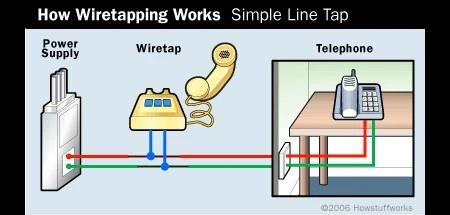
\includegraphics[width=0.85\textwidth]{../../images/python/page_037_img_01.jpeg}

\end{document}
